%%% LaTeX Template: Article/Thesis/etc. with colored headings and special fonts
%%%
%%% Source: http://www.howtotex.com/
%%% Feel free to distribute this template, but please keep to referal to http://www.howtotex.com/ here.
%%% February 2011
%%%
%%% Modified January 2016 by CDM

%%%  Preamble
\documentclass[11pt,letterpaper]{article}
\usepackage[margin=1.0in]{geometry}
\usepackage[T1]{fontenc}
\usepackage[bitstream-charter]{mathdesign}
\usepackage[latin1]{inputenc}					
\usepackage{amsmath}						
\usepackage{xcolor}
\usepackage{cite}
\usepackage{hyphenat}
\usepackage{graphicx}
\usepackage{float}
\usepackage{subfigure}
\usepackage{sectsty}
\usepackage[compact]{titlesec} 
\usepackage[tablegrid]{vhistory}
\usepackage{pbox}
\allsectionsfont{\color{accentcolor}\scshape\selectfont}

%%% Definitions
\definecolor{accentcolor}{rgb}{0.0,0.0,0.5} 
\newcommand{\teamname}{Sound Squad}
\newcommand{\productname}{Sound Vest}
\newcommand{\coursename}{CSE 4316: Senior Design I}
\newcommand{\semester}{Fall 2018}
\newcommand{\docname}{Architectural Design Specification}
\newcommand{\department}{Department of Computer Science \& Engineering}
\newcommand{\university}{The University of Texas at Arlington}
\newcommand{\authors}{Sochima Omenkeukwu \\ Ugo Okoye \\ Jeovanni Santos \\ Anena Sims \\ Connor Twohey}

%%% Headers and footers
\usepackage{fancyhdr}
	\pagestyle{fancy}						% Enabling the custom headers/footers
\usepackage{lastpage}	
	% Header (empty)
	\lhead{}
	\chead{}
	\rhead{}
	% Footer
	\lfoot{\footnotesize \teamname \ - \semester}
	\cfoot{}
	\rfoot{\footnotesize page \thepage\ of \pageref{LastPage}}	% "Page 1 of 2"
	\renewcommand{\headrulewidth}{0.0pt}
	\renewcommand{\footrulewidth}{0.4pt}

%%% Change the abstract environment
\usepackage[runin]{abstract}			% runin option for a run-in title
%\setlength\absleftindent{30pt}			% left margin
%\setlength\absrightindent{30pt}		% right margin
\abslabeldelim{\quad}	
\setlength{\abstitleskip}{-10pt}
\renewcommand{\abstractname}{}
\renewcommand{\abstracttextfont}{\color{accentcolor} \small \slshape}	% slanted text

%%% Start of the document
\begin{document}

%%% Cover sheet
{\centering \huge \color{accentcolor} \sc \textbf{\department \\ \university} \par}
\vspace{1 in}
{\centering \huge \color{accentcolor} \sc \textbf{\docname \\ \coursename \\ \semester} \par}
\vspace{0.5 in}
\begin{figure}[h!]
	\centering
   	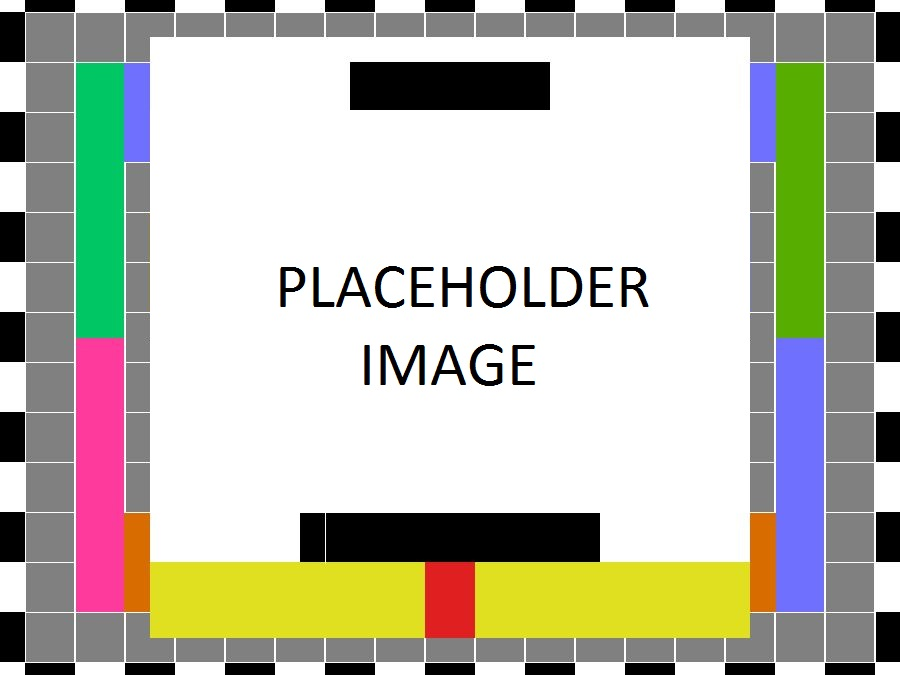
\includegraphics[width=0.60\textwidth]{images/test_image}
\end{figure}
\vspace{0.5 in}
{\centering \huge \color{accentcolor} \sc \textbf{\teamname \\ \productname} \par}
\vspace{0.5 in}
{\centering \large \sc \textbf{\authors} \par}
\newpage


%\vspace{1 in}
%\centerline{January 13th, 2012}
%\newpage

%%% Revision History
\begin{versionhistory}
  	\vhEntry{0.1}{11.20.2018}{AS}{document creation}
  	\vhEntry{0.2}{11.29.2018}{SO|UO|JS|AS|CT}{complete draft}
  	\vhEntry{1.0}{12.04.2018}{SO|UO|JS|AS|CT}{official release}
\end{versionhistory}
\newpage

%%% Table of contents
\setcounter{tocdepth}{2}
\tableofcontents
\newpage

%%% List of figures and tables (optional)
\listoffigures
\listoftables
\newpage

%%% Document sections
\section{Introduction}
The sound backpack will take in a song, filter the low, mid, and high frequencies, then pass those frequencies to different shakers inside the backpack. The shakers will emit a vibration in time with the music so users can feel the beat.

The sound backpack will be available for purchase by the general public, but it will be designed and targeted for customers with hearing disabilities. Age restrictions may apply after evaluating the complexity of the final product.

The backpack will have a simple 2-way switch to serve as the powering on system, as well as a Volume/Intensity Knob and potentiometer for adjusting intensity of the music.
\newpage
\section{System Overview}
Product will be a vest, custom made, from a light weight material. The vest will be one size fits all, with adjustable straps for comfort. Several haptic motor controllers will be strategically sewn into the chest of the vest, along with a micro-controller and button control panel. The motors will vibrate within the vest according to the tempo of music played by the user. The music will be supplied and transmitted to the vest through Spotify API calls. The user will be able to log into the vest’s web based application to select music to play through the vest. The music will play in audio through the device accessing the web app, as well as vibrate through the vest. Profile settings and advanced vest settings can be set in the vest’s web application. The button controls on the vest will allow the customer to make local changes to the function of the vest, like vibration intensity. The vest will receive sound waves and instructions for the motors from a raspberry pi micro controller. The micro-controller will filter through sound waves and send instruction to the motors.
\newpage
\section{Subsystem Definitions \& Data Flow}
This section breaks down your layer abstraction to another level of detail. Here you grapically represent the logical subsytems that compose each layer and show the interactions/interfaces between those subsystems. A subsystem can be thought of as a programming unit that implements one of the major functions of the layer. It, therefore, has data elements that serve as source/sinks for other subsystems. The logical data elements that flow between subsystems need to be explicitly defined at this point, beginning with a data flow-like diagram based on the block diagram.

\begin{figure}[h!]
	\centering
 	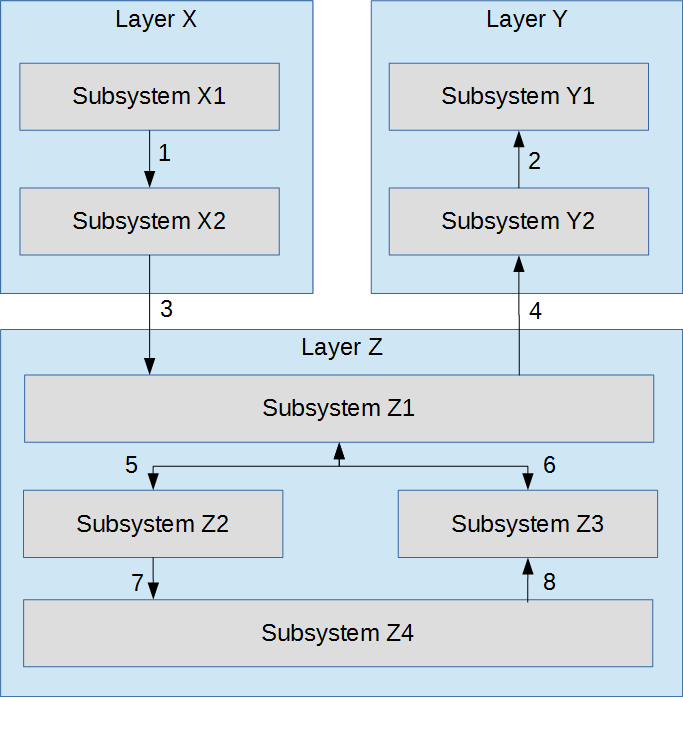
\includegraphics[width=\textwidth]{images/data_flow}
 \caption{A simple data flow diagram}
\end{figure}

\newpage
\section{X Layer Subsystems}
In this section, the layer is described in terms of the hardware and software design. Specific implementation details, such as hardware components, programming languages, software dependencies, operating systems, etc. should be discussed. Any unnecessary items can be ommitted (for example, a pure software module without any specific hardware should not include a hardware subsection). The organization, titles, and content of the sections below can be modified as necessary for the project.

\subsection{Layer Hardware}
A description of any involved hardware components for the layer. For example, if each subsystem is a software process running on an embedded computer, discuss the specifics of that device here. Do not list a hardware component that only exists at the subsystem level (include it in the following sections).

\subsection{Layer Operating System}
A description of any operating systems required by the layer.

\subsection{Layer Software Dependencies}
A description of any software dependencies (libraries, frameworks, etc) required by the layer.

\subsection{Subsystem 1}
Descibe at a high level the purpose and basic design of this subsystem. Is it a piece of hardware, a class, a web service, or something else? Note that each of the subsystem items below are meant to be specific to that subystem and not a repeat of anything discussed above for the overall layer.

\begin{figure}[h!]
	\centering
 	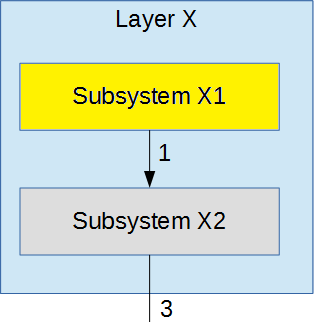
\includegraphics[width=0.60\textwidth]{images/subsystem}
 \caption{Example subsystem description diagram}
\end{figure}

\subsubsection{Subsystem Hardware}
A description of any involved hardware components for the subsystem.

\subsubsection{Subsystem Operating System}
A description of any operating systems required by the subsystem.

\subsubsection{Subsystem Software Dependencies}
A description of any software dependencies (libraries, frameworks, design software for mechanical parts or circuits, etc) required by the subsystem.

\subsubsection{Subsystem Programming Languages}
A description of any programming languages used by the subsystem.

\subsubsection{Subsystem Data Structures}
A description of any classes or other data structures that are worth discussing for the subsystem. For example, data being transmitted from a microcontroller to a PC via USB should be first be assembled into packets. What is the structure of the packets?

\subsubsection{Subsystem Data Processing}
A description of any algorithms or processing strategies that are worth discussing for the subsystem. If you are implementing a well-known algorithm, list it. If it is something unique to this project, discuss it in greater detail.



\newpage
\section{Y Layer Subsystems}
In this section, the layer is described in terms of the hardware and software design. Specific implementation details, such as hardware components, programming languages, software dependencies, operating systems, etc. should be discussed. Any unnecessary items can be ommitted (for example, a pure software module without any specific hardware should not include a hardware subsection). The organization, titles, and content of the sections below can be modified as necessary for the project.

\subsection{Layer Hardware}
A description of any involved hardware components for the layer. For example, if each subsystem is a software process running on an embedded computer, discuss the specifics of that device here. Do not list a hardware component that only exists at the subsystem level (include it in the following sections).

\subsection{Layer Operating System}
A description of any operating systems required by the layer.

\subsection{Layer Software Dependencies}
A description of any software dependencies (libraries, frameworks, etc) required by the layer.

\subsection{Subsystem 1}
Descibe at a high level the purpose and basic design of this subsystem. Is it a piece of hardware, a class, a web service, or something else? Note that each of the subsystem items below are meant to be specific to that subystem and not a repeat of anything discussed above for the overall layer.

\begin{figure}[h!]
	\centering
 	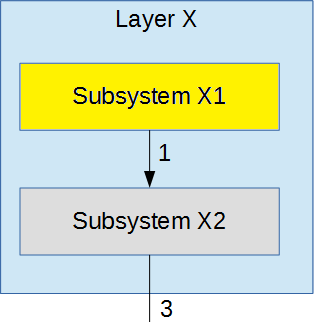
\includegraphics[width=0.60\textwidth]{images/subsystem}
 \caption{Example subsystem description diagram}
\end{figure}

\subsubsection{Subsystem Hardware}
A description of any involved hardware components for the subsystem.

\subsubsection{Subsystem Operating System}
A description of any operating systems required by the subsystem.

\subsubsection{Subsystem Software Dependencies}
A description of any software dependencies (libraries, frameworks, design software for mechanical parts or circuits, etc) required by the subsystem.

\subsubsection{Subsystem Programming Languages}
A description of any programming languages used by the subsystem.

\subsubsection{Subsystem Data Structures}
A description of any classes or other data structures that are worth discussing for the subsystem. For example, data being transmitted from a microcontroller to a PC via USB should be first be assembled into packets. What is the structure of the packets?

\subsubsection{Subsystem Data Processing}
A description of any algorithms or processing strategies that are worth discussing for the subsystem. If you are implementing a well-known algorithm, list it. If it is something unique to this project, discuss it in greater detail.



\newpage
\section{Z Layer Subsystems}
In this section, the layer is described in terms of the hardware and software design. Specific implementation details, such as hardware components, programming languages, software dependencies, operating systems, etc. should be discussed. Any unnecessary items can be ommitted (for example, a pure software module without any specific hardware should not include a hardware subsection). The organization, titles, and content of the sections below can be modified as necessary for the project.

\subsection{Layer Hardware}
A description of any involved hardware components for the layer. For example, if each subsystem is a software process running on an embedded computer, discuss the specifics of that device here. Do not list a hardware component that only exists at the subsystem level (include it in the following sections).

\subsection{Layer Operating System}
A description of any operating systems required by the layer.

\subsection{Layer Software Dependencies}
A description of any software dependencies (libraries, frameworks, etc) required by the layer.

\subsection{Subsystem 1}
Descibe at a high level the purpose and basic design of this subsystem. Is it a piece of hardware, a class, a web service, or something else? Note that each of the subsystem items below are meant to be specific to that subystem and not a repeat of anything discussed above for the overall layer.

\begin{figure}[h!]
	\centering
 	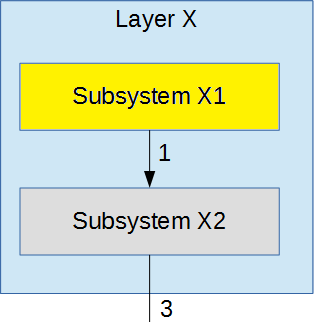
\includegraphics[width=0.60\textwidth]{images/subsystem}
 \caption{Example subsystem description diagram}
\end{figure}

\subsubsection{Subsystem Hardware}
A description of any involved hardware components for the subsystem.

\subsubsection{Subsystem Operating System}
A description of any operating systems required by the subsystem.

\subsubsection{Subsystem Software Dependencies}
A description of any software dependencies (libraries, frameworks, design software for mechanical parts or circuits, etc) required by the subsystem.

\subsubsection{Subsystem Programming Languages}
A description of any programming languages used by the subsystem.

\subsubsection{Subsystem Data Structures}
A description of any classes or other data structures that are worth discussing for the subsystem. For example, data being transmitted from a microcontroller to a PC via USB should be first be assembled into packets. What is the structure of the packets?

\subsubsection{Subsystem Data Processing}
A description of any algorithms or processing strategies that are worth discussing for the subsystem. If you are implementing a well-known algorithm, list it. If it is something unique to this project, discuss it in greater detail.



\newpage

%%% References
\bibliographystyle{plain}
\bibliographystyle{reference/IEEEtran_custom}
\bibliography{reference/refs}{}

\end{document}